% !TEX root = ../dissertacao.tex
\acresetall{}
\chapter{Introdução}
\label{cap:introducao}

\textit{Game engines} contemporâneas devem lidar eficientemente com enormes quantidades de dados para renderizar gráficos 3D em imagens de altíssima resolução, modelar sistemas físicos realistas e também processar sistemas complexos de inteligência artificial.
Para atender a esses requisitos, vários conceitos e padrões de projetos são aplicados durante o desenvolvimento de um jogo para explorar as arquiteturas modernas de computadores, onde o acesso a memória representa o principal gargalo. 
Um dos conceitos empregados durante o desenvolvimento de \textit{game engines} é chamado de \ac{dod}. 
Ao contrário do tradicional \ac{ood}, que se concentra em como os objetos modelam as entidades do problema, o \ac{dod} foca em como os dados serão organizados na memória. 
Esse modelo de programação pode reduzir a complexidade do \textit{software} e visa um processamento mais eficiente, explorando os recursos disponíveis do computador, como por exemplo os recursos de subsistema de memória e a capacidade de multiprocessamento.

O modelo tradicional \ac{ood} faz uso intensivo de herança entre as classes de objetos.
Esta herança tende a criar hierarquias de classes complexas, dificultando a manutenção do \textit{software}~\cite{nystrom2014game}. 
Embora o modelo \ac{dod} possa diminuir essa limitações, a modelagem das estruturas e relações complexas não são tão naturais quanto no modelo \ac{ood}.
Portanto, um padrão de projeto chamado \textit{Entity-Component System} é amplamente adotado no desenvolvimento de \textit{game engines} para lidar eficientemente com a criação e destruição de entidades, e também para gerenciar seus dados subjacentes (denominados de propriedades) \cite{wiebusch2015decoupling, zu2014campvis}.
Este sistema também pode substituir árvores de herança por relações simples, como agregação e composição, para construir um \textit{software} mais robusto e modular.

% problema de hierarquia de classes
Para ilustrar alguns problemas do uso intensivo de herança proporcionado pelo modelo \ac{ood}, vamos tomar como exemplo o desenvolvimento de uma biblioteca de síntese física (\textit{Physical Design}) que deve fornecer informações para  solucionar diferentes problemas pertencentes as etapas de projeto de um \ac{ic}. 
Da mesma forma que as \textit{game engines}, as ferramentas de síntese física devem ser capazes de lidar com um grande volume de dados com um curto tempo de execução.
Adicionalmente, o prazo entre o projeto e a fabricação de um chip é cada vez mais limitado para que um novo produto eletrônico possa garantir o mercado (\textit{time-to-market})~\cite{papa2011physical}.
% Esta biblioteca de síntese física deve fornecer informações para  solucionar diferentes problemas pertencentes a síntese física de um \ac{ic}.
Entre os problemas solucionado por uma biblioteca de síntese física está a estimativa do comprimento de uma interconexão entre duas portas lógicas.
A Figura~\ref{subfig:circuit_example} apresenta um exemplo do um circuito digital contendo duas portas lógicas (A e B), quatro interconexões (N1 a N4) e oito pinos (P1 a P8).

\begin{figure}[ht]
    \centering
    \subfigure[]{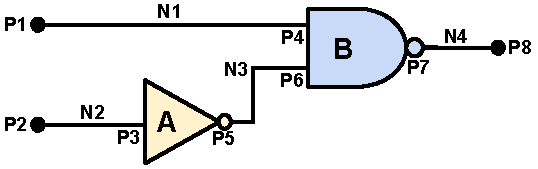
\includegraphics[width=0.6\linewidth]{img/introducao/circuitExample.pdf} \label{subfig:circuit_example}}
    
    \subfigure[]{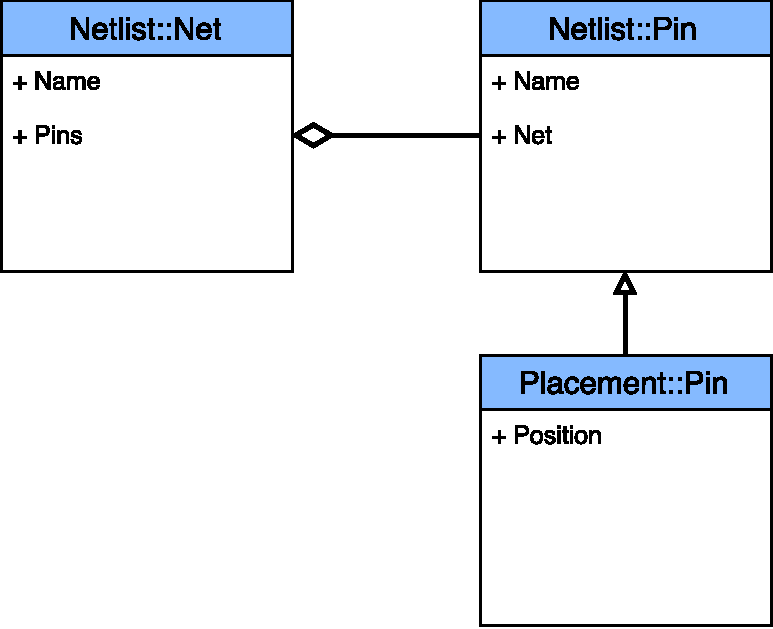
\includegraphics[width=0.38\linewidth]{img/introducao/classHierarchyOOD.pdf} \label{subfig:classHierarchyOOD}}
    \hspace{0.5cm}
    \subfigure[]{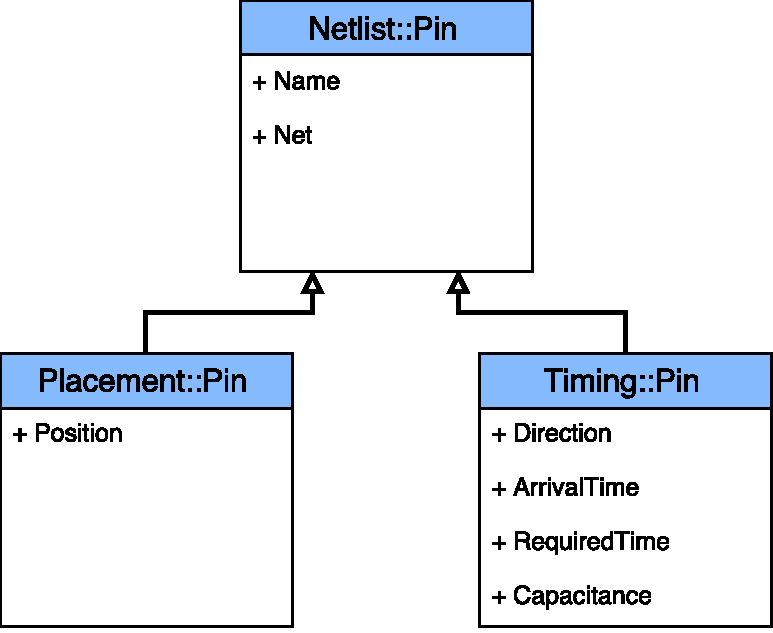
\includegraphics[width=0.38\linewidth]{img/introducao/classHierarchyTimingOOD.pdf} \label{subfig:classHierarchyTimingOOD}}
    \caption[Exemplo de um circuito digital]{Exemplo de um circuito digital e seu diagrama de classe para o problema de estimar o comprimento de uma interconexão.}
    \label{fig:circuit_example}
\end{figure}

Uma possível decomposição para a estimativa do comprimento de interconexão com o modelo \ac{ood} é apresentada na Figura~\ref{subfig:classHierarchyOOD}.
Este diagrama de classe representa dois módulos: \textit{netlist} e \textit{placement}
O módulo \textit{netlist} possui duas classes, \textit{net} e \textit{pin}, para descrever as interconexões do circuito e os pinos associados, respectivamente.
Para a classe \textit{pin}, este módulo caracteriza apenas o nome do pino e a interconexão a que esse pino pertence, sem nenhuma informação de posicionamento.
O módulo \textit{placement}, por sua vez, descreve as posições dos pinos.
A seta com ponta de diamante entre as classes \textit{pin} e \textit{net} representa uma relação de agregação, o que significa que uma interconexão possui
referência aos seus pinos, enquanto um pino possui referência à interconexão a qual ele pertence. A seta de ponta triangular entre as duas classes \textit{pin} representa um relacionamento de hierarquia, o que significa que a classe \textit{pin} do módulo \textit{placement} estende os atributos da classe \textit{pin}
classe no módulo \textit{netlist}.

Porém, quando algum problema necessitar de informações da temporização dos pinos, a classe \textit{pin} do módulo \textit{netlist} apresentada na Figura~\ref{subfig:classHierarchyOOD} deverá ser estendida para possuir estas informações. Esta nova hierarquia de classe é apresentada na Figura~\ref{subfig:classHierarchyTimingOOD}.
Contudo, problemas que necessitem de informações de posicionamento e temporização (como por exemplo algoritmos de \textit{timing-driven placement} (ITDP)) deverão possuir informações de posicionamento e tempo.
Em \ac{ood}, isso pode ser feito através de herança múltipla, onde uma nova classe \textit{pin} estende as classes \textit{pin} dos módulos \textit{placement} e \textit{timing}.
No entanto, a herança múltipla não é suportada por todas as linguagens de programação e, mesmo quando suportada, não é recomendada
porque isso pode levar a problemas de design~\cite{nystrom2014game}.

\begin{figure}[h!b]
    \centering
    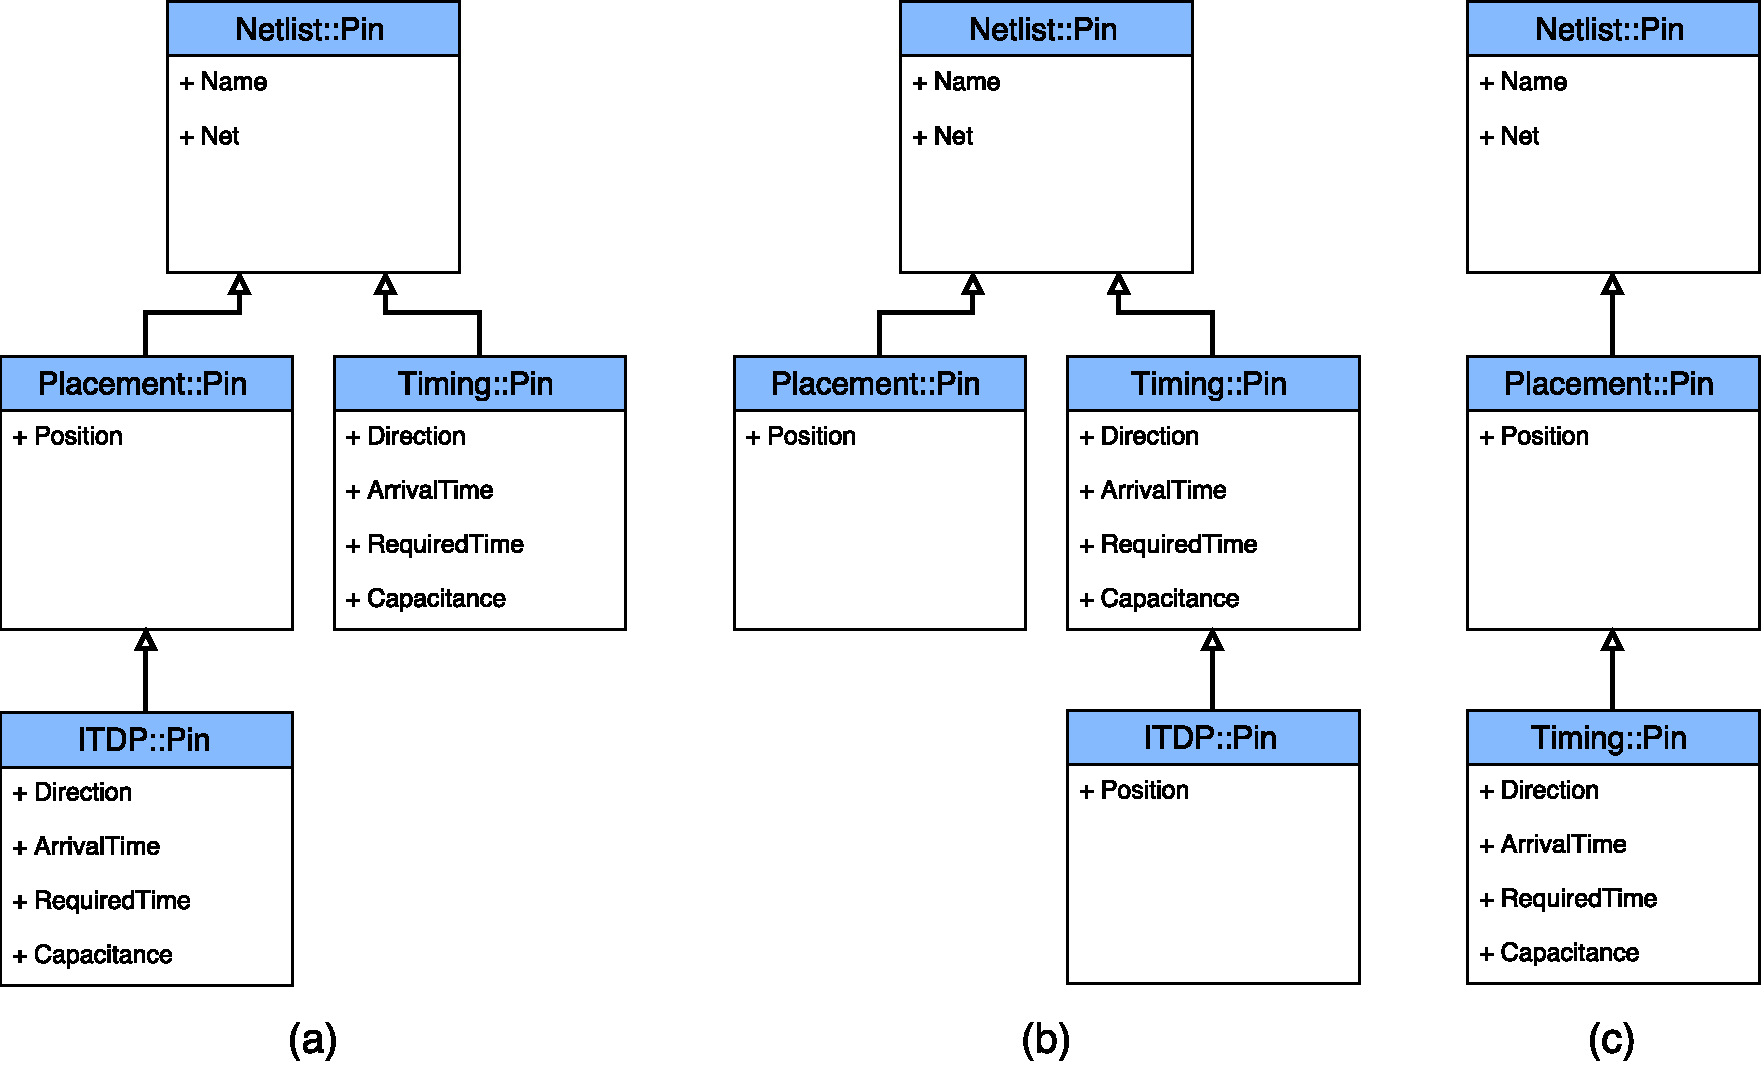
\includegraphics[width=0.8\textwidth]{img/introducao/ITDPsolutionOOD.pdf}
    % \caption{Class Hierarchy OOD.}
    \caption[Hierarquia de classes]{Possível hierarquia de classes para suportar informações de posicionamento e tempo para um algoritmo de \textit{timing-driven placement} utilizando o  modelo \ac{ood}.}
    \label{fig:classITDP}
\end{figure}

Sem recorrer à herança múltipla, a solução consiste em criar uma nova classe \textit{pin} que se estende a partir do módulo \textit{placement} ou \textit{timing} e possui repetição do código da outra classe (que não foi estendida). As Figuras~\ref{fig:classITDP} (a) e (b) mostram essas duas soluções. De qualquer forma, não há maneira simples de reutilizar informações de posicionamento e tempo sem ocorrer replicação de informações. A única opção que resta é juntar todas as informações na classe \textit{pin} do módulo \textit{timing} fazendo com que estenda a classe \textit{pin} do módulo \textit{placement}. Esta solução é ilustrada na Figura~\ref{fig:classITDP} (c). No entanto, nem sempre é necessário ter informações de posicionamento no módulo \textit{timing}. Por exemplo, uma ferramenta de \ac{sta} pode não precisar de informações de posicionamento durante as primeiras etapas de design. Portanto, a adoção da última solução levaria ao desperdício da localidade espacial da memória \textit{cache}, já que informações desnecessárias seriam recuperadas juntamente com informações úteis.




% conexão game engine com EDA

% Da mesma forma que as \textit{game engines}, as ferramentas de \ac{eda} devem ser capazes de lidar com um grande volume de dados com um curto tempo de execução.
% Adicionalmente, o prazo entre o projeto e a fabricação de um chip é cada vez mais limitado para que um novo produto eletrônico possa garantir o mercado (\textit{time-to-market})~\cite{papa2011physical}.
% Para isso, estas ferramentas devem empregar otimizações de \textit{software}, como o uso de melhores organizações nos dados, estruturas de dados otimizadas, paralelização e exploração da localidade de dados na \textit{cache}.
Para garantir a execução dentro de tempos de execução aceitáveis, as ferramentas \ac{eda} devem aproveitar ao máximo as otimizações de software, como: uso de estruturas de dados otimizadas, paralelização e exploração da localidade da memória \textit{cache}.
Se examinarmos as ferramentas atuais \ac{eda} disponibilizadas pela academia, como as obras de \cite{universityOfMichigan, kahng2014horizontal, jung2016opendesign, flach2017rsyn, openAccess}, todos eles realizam uma série de otimizações de software, mas nenhum deles se concentra na organização de dados para explorar a localidade espacial da memória \textit{cache}.
Já os trabalhos que focam na exploração da localidade espacial e temporal dos dados, como \cite{li2014, Tang2015, qasem2017characterizing}, não realizam avaliações no contexto da síntese física.
Portanto, este trabalho se concentra na discussão e aplicação desses conceitos modernos de engenharia de  \textit{software} visando o desenvolvimento de ferramentas para a síntese física.

\section{Justificativa}

    Apesar de vários trabalhos encontrados na literatura fazerem otimizações de \textit{software} mencionadas na seção anterior, nenhum deles avalia o impacto destas diferentes estratégias quando aplicadas no contexto da síntese física.

    % Portanto, é desejável uma análise quantitativa do impacto da organização dos dados no contexto de Physical Design, sobretudo, com uma comparação que faça uso de uma infraestrutura realista e bem consolidada na academia.
    Portanto, é desejável uma análise quantitativa do impacto da organização dos dados no contexto da síntese física, sobretudo, com um estudo de problemas reais utilizando entradas realistas para a experimentação.

\section{Objetivos e Contribuições Alcançadas}

    Este trabalho tem como objetivo a avaliação quantitativa do impacto causado pela organização dos dados em diferentes algoritmos no contexto da síntese física

    Os objetivos específicos deste trabalho são:

    \begin{itemize}
        \item Implementar um conjunto de algoritmos de Physical Design que possuam diferentes características;
        \item Avaliar as organizações dos dados propostas comparando-as com a modelagem tradicional utilizada, resultante do uso de orientação a objetos. A comparação será realizada comparando o número de \textit{cache misses} gerados pelas implementações dos algoritmos, bem como o tempo de execução;
        \item Investigar possíveis otimizações na organização dos dados, como por exemplo o ordenamento dos mesmos, para cada algoritmo implementado;
        \item Avaliar o desempenho da paralelização dos algoritmos implementados com as diferentes organização dos dados.
    \end{itemize}

\section{Contribuições científicas e tecnológicas}

    Este trabalho traz as seguintes contribuições científicas e tecnológicas:

    \begin{itemize}
        \item Implementação de um sistema de componentes e entidades. Estes conceitos serão detalhados na Seção~\ref{sec:entity_component_system} desta dissertação;
        \item Avaliação quantitativa do desempenho gerado pela modelagem dos dados em algoritmos pertencentes a síntese física;
        \item Resultados experimentais utilizando uma infraestrutura baseada em circuitos industriais. Como dados de entrada serão utilizados circuitos industriais oriundos da competição ICCAD CAD Context 2015~\cite{kim2015};
        \item Comparação quantitativa do número de \textit{cache misses} e o tempo de execução para quatro algoritmos da síntese física.  
    \end{itemize}


% \section{Metodologia}
%         Implementar versões de problemas
%         avaliar quantitativamente o número de cache misses
%         avaliar quantitativamente o tempo de execução
%
% \section{Limitações(escopo) deste trabalho}
%         somente 3 problemas avaliados
%         somente uma arquitetura de processador e cache
%         paralelização com um chunk único

% \section{Organização deste trabalho}
\section{Organização deste trabalho}

O Capítulo~\ref{cap:conceitos_fundamentais} revisa alguns conceitos fundamentais para a melhor compreensão deste trabalho.
No Capítulo~\ref{cap:trabalhos_correlatos} são apresentados os trabalhos correlatos na otimização da organização dos dados para uma melhor utilização da \textit{cache}.
O Capítulo~\ref{cap:tecnica_proposta} descreve a proposta de organização dos dados e seus possíveis impactos para o contexto de Physical Design.
O Capítulo~\ref{cap:caracterizacaoSinteseFisica} caracteriza os algoritmos presentes na etapa de síntese física do fluxo de projeto de \acp{ic}.
No Capítulo~\ref{cap:resultados} são apresentadas as organizações dos dados utilizadas para cada estudo de caso e os resultados experimentais.
Por fim, o Capítulo~\ref{cap:conclusao_e_trabalhos_futuros} apresenta as conclusões obtidas com a realização deste trabalho e as possíveis extensões deste trabalho.

